%% Bookheader, Nov 8, 2020; July 18, 2022

\documentclass[11pt]{../Support/ourbook}
%% or for landscape, comment out line above and use this one:
%%\documentclass[landscape,11pt]{ourbook}

%% This will keep space from stretching around display math:

\makeatletter
\renewcommand\normalsize{%
   \@setfontsize\normalsize\@xipt{13.6}%
   \abovedisplayskip 11\p@  \@minus6\p@
   \abovedisplayshortskip \z@ 
   \belowdisplayshortskip 6.5\p@ \@minus3\p@
   \belowdisplayskip \abovedisplayskip
   \let\@listi\@listI}
\makeatother
\normalsize


\begin{document}

\tableofcontents
\graphicspath{{../../Chapters/dc1/en_US}}
\chapter{Introduction to Electricity}

What happens when you turn on a flashlight? The battery in the
flashlight acts as an electron pump. The electrons flow through the
wires to the lightbulb (or LED). As the electrons pass through the
lightbulb, they excite the molecules within, which gives off light and
heat. (LEDs also give off light and heat, but they give off a lot less
heat.) Then the electrons return to the battery to be pumped around
again.

When electricity is flowing through a copper wire, the protons and
neutrons of the copper stay put while the electrons jump between the
atoms on their way from the battery to the lightbulb and back again.

In some materials, like copper and iron, electrons are loosely bound
to their nuclei, forming a sea of electrons, which allows energy to flow. These are good \textit{electrical conductors}. In
other materials, like glass and plastic, electrons don't leave their
nuclei easily. Thus, they are terrible electrical conductors -- we call
them \textit{electrical insulators}. For example, the plastic around a
wire is electrical insulation.

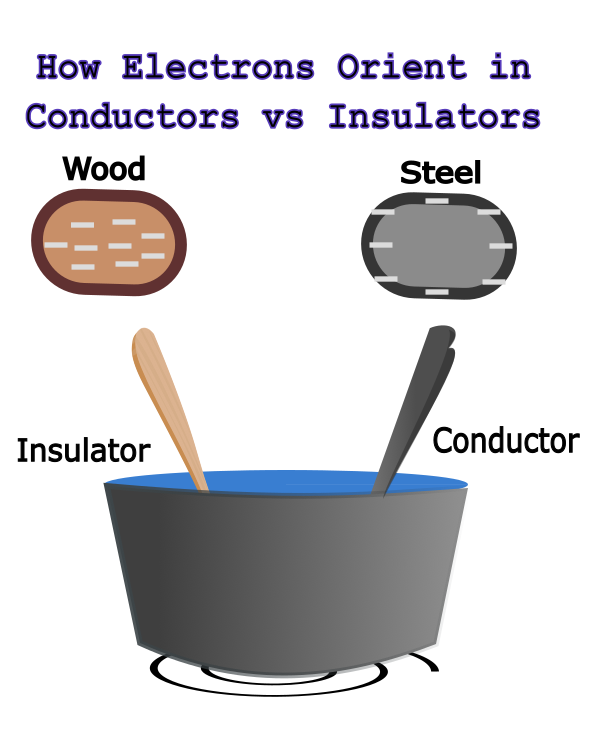
\includegraphics[width=0.8\textwidth]{Insulator_vs_Conductor.png}
% KA: https://www.khanacademy.org/science/physics/electric-charge-electric-force-and-voltage/charge-electric-force/v/conductors-and-insulators

\section{Units}

Electrons are very small, so to study them, scientists came up with a
unit that represents \textit{a lot} of electrons. 1 \textit{coulomb}
is about 6,241,509,074,460,762,608 electrons.  When 5 coulombs enter one end of the wire every second (and simultaneously 5 coulombs exit the other end), we say ``This wire is carrying 5 amperes of current.''\index{coulombs}

(Truthfully, we usually shorten ampere to just ``amp''.  This is
sometimes a little awkward because we often shorten the word
``amplifier'' to ``amp''. You should be able to tell which is which
from the context.)\index{amp or ampere}

If you look at the circuit breakers or fuses for your home's
electrical system, you'll see that each one is rated in amps.  For
example, maybe the circuit that supplies power to your kitchen has a 10
amp circuit breaker. If for some reason, more than 10 amps tries to
pass through that wire, the circuit breaker will turn off the whole
circuit.

When it is on, your flashlight pushes about 1 amp of current
through the lightbulb(When it is off, there is no current in the
lightbulb).

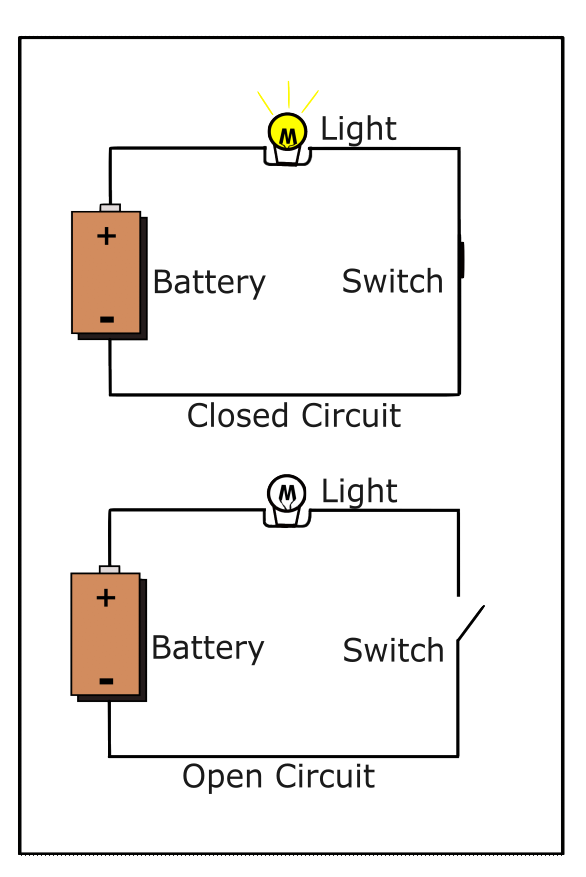
\includegraphics[width=0.8\textwidth]{Circuit_OnOff.png}

The lightbulb creates \textit{Resistance} that the current pushes
through.\index{resistance} Think of it like plumbing: The current is the amount of water
passing through a pipe. The resistance is something that tries to stop
the current -- like a ball of hair. The battery is what allows
 the current to push through the resistance; we call that
pressure \textit{voltage}.\index{voltage}

\section{Circuit Diagrams}

Here is a circuit diagram of your flashlight:

\begin{circuitikz}
\draw (0,0) to[battery1,invert,l=$3V$] ++(0,3)
to [switch,i=1A] ++(3,0)
to [lamp=$1\Omega$,bipoles/length=0.9cm] ++(0,-3) -- (0,0);
\end{circuitikz}

The lines are wires.  The symbols that we  will use:

\begin{tabular}{c c c c}
  Battery & Switch & Lamp & Resistor \\
\begin{circuitikz}
\draw (0,0) to[battery1] (2,0); 
\end{circuitikz}
&
\begin{circuitikz}
\draw (0,0) to[lamp,bipoles/length=0.9cm,l=$3 \Omega$] (2,0); 
\end{circuitikz}
&
\begin{circuitikz}
\draw (0,0) to[switch,/tikz/circuitikz/bipoles/length=1.0cm] (2,0); 
\end{circuitikz}
&
\begin{circuitikz}
\draw (0,0) to[R,  l=$3 \Omega$] (2,0); 
\end{circuitikz} \\
\end{tabular}

The battery pushes the electrons from one end and pulls them back in at the other, so the circuit must go around in a circle for the current to flow. This is why the current stops flowing when the switch breaks the circuit.

You can think of a switch as having zero resistance when it is closed and infinite resistance when it is open.


For our purposes, a lamp is just a resistor that gives off light.
% KA: https://www.khanacademy.org/science/high-school-physics/dc-circuits/electric-power-and-dc-circuits/a/circuit-introduction

\section{Ohm's Law}

Resistance is measured in \textit{ohms}, and we use a Greek capital omega for that: $\Omega$  

Voltage is measured in
\textit{volts}.\index{ohms}\index{volts}

\begin{mdframed}[style=important, frametitle={Ohm's Law}]\index{Ohm's law}
  Whenever a voltage $V$ is pushing a current $I$ through a resistance of $I$, the following is true:

  $$V = IR$$

  where $V$ is in volts, $I$ is in amps, and $R$ is in ohms.
\end{mdframed}
% KA: https://www.khanacademy.org/science/physics/circuits-topic/circuits-resistance/v/circuits-part-1

\section{Power and Watts}

\begin{mdframed}[style=important, frametitle={Joule's Law}]\index{Joule's law}

  When a current $I$ is passing through a resistance $R$, the power consumed is
  
  $$W = I^2 R$$

  where $W$ is in watts, $I$ is in amps, and $R$ is in ohms.
\end{mdframed}

Of course $V = IR$, so we can extend this to:

$$W = I^2 R = I V = \frac{V^2}{R}$$

Your flashlight's batteries provide about 3 volts. How much
battery power is the flashlight using when it is on? The power (in
watts) produced by the battery is the product of the voltage (in
volts) and the current (in amps). So your flashlight is giving off $3
volts \times 1 amp = 3 watts$ of power. Some of that power is given
off as light, some as heat.\index{watts}

A watt is 1 joule of energy per second. We say that a watt is a
measure of \textit{power}.

When we talk about how much energy is stored in a battery, we use a
unit like a kilowatt-hour. A kilowatt-hour is equivalent to 3.6 million
joules.

\section{Another great use of RMS}

In many electrical problems, the voltage fluctuates a lot.  For
example, the fluctuations in voltage makes the sound that comes out of an
audio speaker.

You can use the root-mean-squared of the voltage to figure out the average power
your speaker is consuming.

Let's say that the RMS of the voltage you are sending to the speaker is $V_{rms}$
and the resistance of the speaker is $R$ ohms, then the power consumed
by the speaker is:

$$P = \frac{V_{rms}^2}{R}$$

Similarly, if you know the RMS of the current you are pushing through
the speaker is $I_{rms}$, then the power consumed by the speaker is:

$$P = I_{rms} R$$

\section{Electricity Dangers}

Large amounts of electricity moving through your body can hurt or even kill
you. You must be careful around electricity.

However, your body is not a very good conductor, so low-voltage
systems (like a flashlight) don't have enough voltage to move significant amounts of
current through your body.

However, the  electricity in a power outlet has much more voltage. The voltage
in these outlets is fluctuating between positive and negative, so we
call it \textit{Alternating Current} or AC.
% ADD: Introduce difference between AC and dc

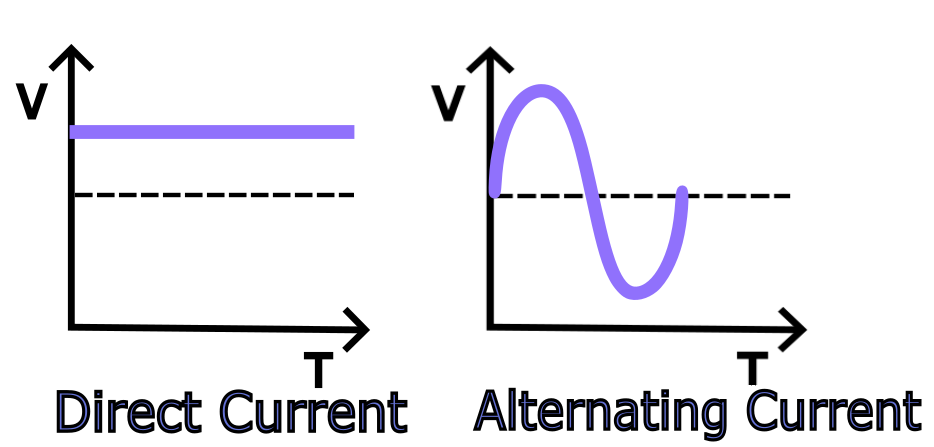
\includegraphics[width=0.8\textwidth]{AC_vs_DC.png}

In most countries, the RMS of the voltage between 110 and 240 V. (The
peak voltage is always $\sqrt{2}$ times the RMS value. In the US, for
example, people say ``Our outlets supply 120 V.'' They mean that the
RMS of the voltage difference between the wire and the earth is 120V.
The peak voltage is almost 170V.)

How much current can a human handle? Not much. You can barely feel 1
mA moving through your body, but at 16 mA, your muscles will clench
and you won't be able to relax them -- many people die from
electrocution because they grab a wire which pushes enough current
through their body to prevent them from letting go of the wire.  At 20
mA, a human's respiratory muscles become paralyzed.

The fuse breaker in a house will often allow 20 A to flow through the
circuit before it shuts off the power: Always, always, always shut off
the power before touching any of the wiring in your house.

While water is actually a mediocre conductor, it can still deliver enough current
to kill you. If you see a wire in a puddle, you should not touch the
puddle. Interestingly, because of the salt, sea water is more than
100 times better at conducting electricity than the water you drink.
% ADD: Sea of electrons makes a good conductor

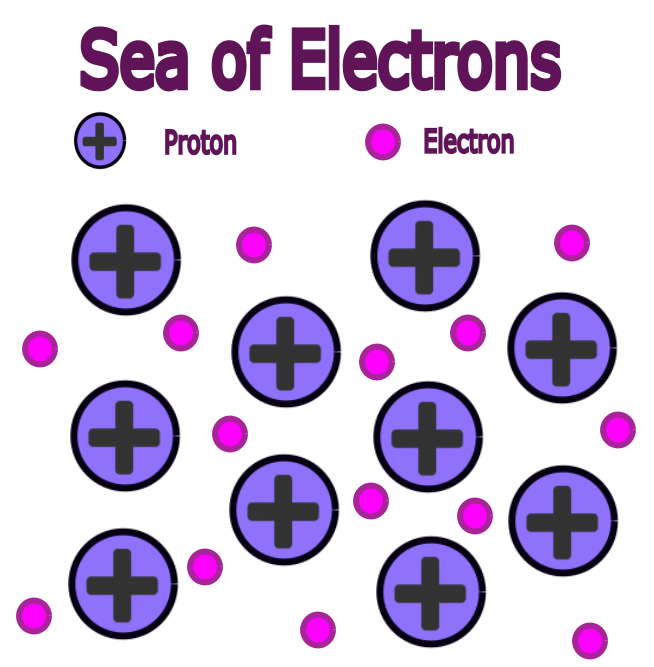
\includegraphics[width=0.8\textwidth]{Sea_Electrons.png}

If you hold a wire in each hand, how many Ohms of resistance will your
body have? Once it gets past your skin, you will look like a bag of
salt water to the electricity. After the skin, your body will have a
resistance of about 300$\Omega$. However, the skin is a pretty good
insulator. If you have dry, calloused hands, your skin may add a
100,000$\Omega$ to the resistance.

% KA: https://www.khanacademy.org/science/in-in-class10th-physics/in-in-electricity/in-in-electric-power-and-heating-effect-of-current/v/electric-power-energy


\graphicspath{{../../Chapters/dc_circuits/en_US}}
\chapter{DC Circuit Analysis}

In the most basic circuit, you have only a battery and a resistor:



\begin{circuitikz}
\draw (0,0) to[battery1,invert,l=$6V$] ++(0,3)
to ++(3,0)
to [R=$3\Omega$, /tikz/circuitikz/bipoles/length=1.0cm,i=2A] ++(0,-3) -- (0,0);
\end{circuitikz}

In this case, you only need Ohm's Law: $V = I R$.  In this case, $6V = 3\Omega \times 2A$.
% ADD: Define Ohm's Law
\begin{Exercise}[title={Ohm's Law}, label=ohms_check]

  How many amps are going around the circuit?
  
  \vspace{1cm}

\begin{circuitikz}
\draw (0,0) to[battery1,invert,l=$24V$] ++(0,3)
to ++(3,0)
to [R=$6\Omega$, /tikz/circuitikz/bipoles/length=1.0cm,i={? A}] ++(0,-3) -- (0,0);
\end{circuitikz}

  
\end{Exercise}
\begin{Answer}[ref=ohms_check]

  $V = I R$ so $I = \frac{V}{R} = \frac{24V}{6\Omega} = 4A$.
  
\end{Answer}
% KA: https://youtu.be/F_vLWkkOETI

\section{Resistors in Series}

When you have two resistors wired together in a long line, we say they
are ``in series''.  If you have two resistors $R_1$ and $R_2$ wired in
series, the total resistance is $R_1 + R_2$.

In this diagram, for example, the total resistance is $5\Omega$.

\begin{circuitikz}
\draw (0,0) to[battery1,invert,l=$10V$] ++(0,5)
to ++(3,0)
to [R=$3\Omega$] ++(0,-2.5)
to [R=$2\Omega$] ++(0,-2.5) -- (0,0);
\end{circuitikz}

The current flowing through the circuit, then, is $10/4 = 2A$.

By Ohm's law, the voltage drop across the upper resistor is $I R = 2A \times 3\Omega = 6V$.

The voltage drop across the lower resistor is $I R = 2A \times 2\Omega = 4V$.

Notice that the battery pumps the voltage up to $10V$, then the two
resistors drop it by exactly $10V$. This is known as ``Kirchhoff's
Voltage Law'':
% KA: https://youtu.be/4rsswT_Rv1M

\begin{mdframed}[style=important, frametitle={Kirchhoff's Voltage Law}]\index{Kirchhoff's voltage law}
As you make a loop around a circuit, the sum of the voltage increase
must equal the sum of the voltage decrease.
\end{mdframed}

The negative end of the battery is connected to ``ground'' (
it has zero voltage), then we can draw a diagram with the
voltages(That symbol in the lower right represents a connection to ground).

\begin{circuitikz}
\draw (0,0) to[battery1,invert,l=$6V$] ++(0,5) 
to [-*] ++(3,0) node[anchor=west] {10V}
to [R=$3\Omega$,-*] ++(0,-2.5) node[anchor=west] {4V}
to [R=$2\Omega$,-*] ++(0,-2.5) node[anchor=west]{0V} node[ground]{} --(0,0);
\end{circuitikz}


\begin{Exercise}[title={Resistors In Series}, label=series_resistor]

  What is the current going around the circuit?
  
  What is the voltage drop across each resistor?
  
  \vspace{1cm}
\begin{circuitikz}
\draw (0,0) to[battery1,invert,l=$16V$] ++(0,5) 
to [-*] ++(3,0) node[anchor=west] {16V}
to [R=$5\Omega$,-*] ++(0,-2.5) node[anchor=west] {?}
to [R=$3\Omega$,-*] ++(0,-2.5) node[anchor=west]{0V} node[ground]{} --(0,0);
\end{circuitikz}


\end{Exercise}
\begin{Answer}[ref=series_resistors]

  There is a total resistance of $8\Omega$, so your 16V will push 2A
  of current around the circuit.

  2A going through a $5\Omega$ resistor represents a 10V drop.

  2A going through a $3\Omega$ resitor represents a 6V drop.
  
\end{Answer}


\section{Resistors in Parallel}

Look at this circuit. Note that the current can go two different paths.

\begin{circuitikz}
\draw (0,0) to[battery1,invert,l=$12V$] ++(0,3)
to ++(3,0)
to [R=$2\Omega$, /tikz/circuitikz/bipoles/length=1.0cm] ++(0,-3) -- (0,0);
\draw (3,3) -- (5,3)
to [R=$3\Omega$, /tikz/circuitikz/bipoles/length=1.0cm] ++(0,-3) -- (3,0);
\end{circuitikz}

There is 12 volts pushing current through both resistors. So 6A will
go through the 2$\Omega$ resistor and 4A will go through the 3$\Omega$
resistor.

\begin{circuitikz}
\draw (0,0) to[battery1,invert,l=$12V$] ++(0,3)
to ++(3,0)
to [R=$2\Omega$, /tikz/circuitikz/bipoles/length=1.0cm,i=6A] ++(0,-3) -- (0,0);
\draw (3,3) -- (5,3)
to [R=$3\Omega$, /tikz/circuitikz/bipoles/length=1.0cm,i=4A] ++(0,-3) -- (3,0);
\end{circuitikz}

Thus, a total of 10 A will be going through the battery.

Imagine you are a battery. You can't see that you have two resistors.
What does it feel like to you? $\frac{V}{I} = R$, and $V= 12$ and $I =
10$.  So the effective resistance of the two resistors in parallel is
$\frac{12}{10}$ or $\frac{6}{5} \Omega$.

\begin{mdframed}[style=important, frametitle={Resistance in Parallel}]\index{resistance!in parallel}
If you have several resistances $R_1, R_2, \ldots, R_n$ wired in
parallel, their effective resistance $R_t$ is given by

$$\frac{1}{R_t} = \frac{1}{R_1} + \frac{1}{R_2} + \ldots + \frac{1}{R_n}$$

\end{mdframed}

In our example:

$$\frac{1}{R_t} = \frac{1}{2} + \frac{1}{3} = \frac{5}{6}$$

Thus $R_t =  \frac{6}{5}\Omega$.

\begin{Exercise}[title={Resistors In Parallel}, label=parallel_resistors]

  What is the current going through the battery?
  What is the drop over the $4\Omega$ resistor?
  What is the current in each branch?

  \vspace{1cm}

  \begin{circuitikz}
\draw (0,0) to[battery1,invert,l=$12V$] ++(0,3)
to [R=$4\Omega$, /tikz/circuitikz/bipoles/length=1.0cm] ++(3,0) node [yshift=0.3cm] {? V}
to [R=$6\Omega$, /tikz/circuitikz/bipoles/length=1.0cm,i={? A}] ++(0,-3) node[ground]{} -- (0,0);
\draw (3,3) -- (5,3)
to [R=$3\Omega$, /tikz/circuitikz/bipoles/length=1.0cm,i={? A}] ++(0,-3) -- (3,0);
\end{circuitikz}

\end{Exercise}
\begin{Answer}[ref=parallel_resistors]
  The effective resistance of the $6\Omega$ and the $3\Omega$ is $2\Omega$ because 

  $$\frac{1}{R_T} = \frac{1}{6} + \frac{1}{3} == \frac{1}{2}$$

  So the battery experiences a resistance of $4\Omega + 2\Omega =
  6\Omega$.  A $12V$ will push 2A through a resistance of $6\Omega$.

  The voltage drop across the $4\Omega$ resistor is $2A \times 4\Omega
  = 8V$. Thus there will be a 4V drop across the two resistors in
  parallel.  So 2/3 A will flow through the $6\Omega$ resistor. 4/3 A
  will flow through the $3\Omega$ resistor.

    \begin{circuitikz}
\draw (0,0) to[battery1,invert,l=$12V$] ++(0,3)
to [R=$4\Omega$, /tikz/circuitikz/bipoles/length=1.0cm] ++(3,0) node [yshift=0.3cm] {8 V}
to [R=$6\Omega$, /tikz/circuitikz/bipoles/length=1.0cm,i={2/3 A}] ++(0,-3) node[ground]{}-- (0,0);
\draw (3,3) -- (5,3)
to [R=$3\Omega$, /tikz/circuitikz/bipoles/length=1.0cm,i={4/3 A}] ++(0,-3) -- (3,0);
\end{circuitikz}
  
\end{Answer}


\graphicspath{{../../Chapters/charge/en_US}}
\chapter{Charge}

If you rub a balloon against your hair and then place it next to a wall it will stick. We
say that it has gotten an \textit{electrical charge}. It stole some
electrons from your hair, and now the ballon has slightly more
electrons than protons. We say that it has a negative electrical
charge.

Objects with slightly more protons than electrons have a positive charge.

This charge is measured in coulombs. The charge of a single proton is
about $1.6 \times 10^{-19}$ coulombs.

An object with a negative charge and an object with a positive charge
will be attracted to each other. Two objects with the same charge will
be repelled by each other.
% ADD: Good place for culloms law
% KA: https://www.khanacademy.org/science/hs-physics/x215e29cb31244fa1:types-of-interactions/x215e29cb31244fa1:coulomb-s-law/v/coulombs-law

\begin{mdframed}[style=important, frametitle={Coulomb's Law}]\index{Coulomb's law}

  If two objects with charge $q_1$ and $q_2$ (in coulombs) are $r$ meters from each other, the force of attraction or repulsion is given by

  $$F = K\frac{\lvert q_1 q_2 \rvert}{r^2}$$

    where $F$ is in newtons and $K$ is Coulomb's constant: about $8.988 \times 10^9$.
  
\end{mdframed}


\begin{Exercise}[title={Coulomb's Law}, label=charged_balloons]

Two balloons are charged with an identical quantity and type of
charge: $-5 \times 10^{-9}$ coulombs. They are held apart at a
separation distance of 12 cm. Determine the magnitude of the
electrical force of repulsion between them. 
  
\end{Exercise}
\begin{Answer}[ref=charged_balloons]

  $$F = K\frac{\lvert q_1 q_2 \rvert}{r^2} = (8.988 \times 10^9) \frac{(-5 \times 10^{-9})(-5 \times 10^{-9})}{0.12^2} = \frac{224.7 \times 10^{-9}}{0.0144} = 15.6 \times 10^{-6}$$

  15.6 micronewtons.
  
\end{Answer}

At this point, you might ask ``If the wall has zero
charge, why is the balloon attracted to it?'' The answer: the
electrons in the wall move away from the balloon. The negative charge
on the balloon pushes electrons into the wall, so the surface of the
wall gets a mild positive charge. The surface is close to the balloon,
so the attraction is stronger than the repulsion.

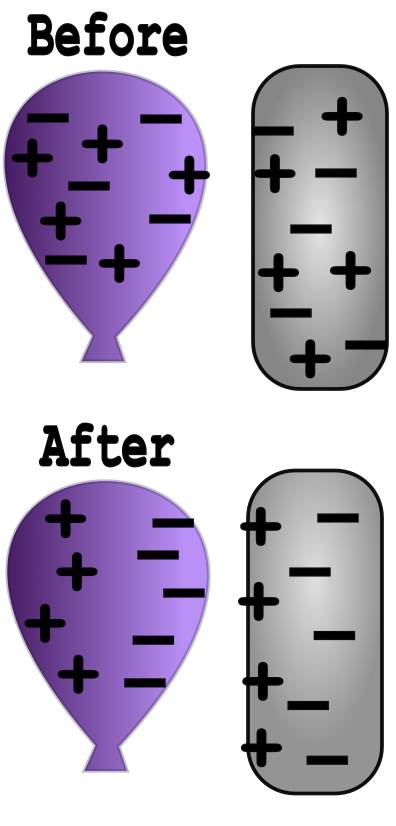
\includegraphics[width=0.4\textwidth]{Ballon_Diagram.png}

\section{Lightning}

A cloud is a cluster of water droplets and ice particles. These
droplets and ice particles are always moving up and down through the
cloud. In this process, electrons get stripped off and end up on the
water droplets at the bottom of the cloud( water droplets collect at the bottom because they are denser). The air between the
droplets is a pretty good insulator, and thus the electrons are reluctant
to jump anywhere. However, eventually, the charge gets so strong that
even the insulating properties of the air is not enough to prevent
the jump, causing lightning.
% ADD: Add water density explanation. ice less dense than liquid water due to crystaline structure.

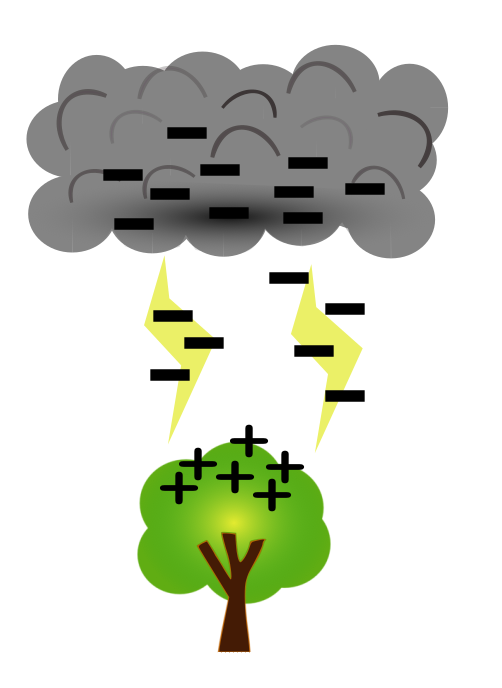
\includegraphics[width=0.8\textwidth]{Lighting_Diagram.png}

A lot of lightning moves within a cloud or between clouds. However, a
few jump to the earth. These bolts of lightning vary in the amount of
electrons they carry, but the average is about 15 coulombs.

And thunder occurs because the electrons heat the air they pass through, 
causing the air to expand suddenly, and the resulting shockwave is the sound we know as thunder.
% ADD: Relate speed of light and sound 
\section{But...}

This idea that opposite charges attract creates some heavy questions
that you do not yet have the tools to work with. So the answer is
basically ``Don't ask that question now!''

However, you probably have these questions, so I will point you in
the direction of the answers.

The first is ``In any atom bigger than hydrogen, there are multiple
protons in the nucleus. Why don't the protons push each other out of
the nucleus?''

We aren't ready to talk about it, but there is a force called \textit{the
 nuclear force} which pulls the protons and neutrons in the nucleus
of the atom toward each other. At very, very small distances it is
strong enough to overpower the repulsive force due to the protons'
charges.
% ADD: Effective nuclear charge

Another question is ``Why do the electrons whiz around in a cloud so
far from the nucleus of the atom? Negatively charged electrons should
cling to the protons in the center, right?''

We aren't ready to talk about it, but quantum mechanics tells us that
electrons like to live in a certain specific energy level. Hugging
protons isn't one of those levels.

\graphicspath{{../../Chapters/fertilizer/en_US}}
\chapter{Fertilizer}

In 1950, there were 2.5 billion people on the planet, and about 65\%
were malnourished. In 2019, there were 7.7 billion people on the
planet, and only 15\% are malnourished. How did crop yields increase
so much? There were several factors: better crop varieties,
reliable irrigation, increased mechanization, and affordable fertilizers.\index{fertilizer}

When a plant grows, it takes molecules out of the soil and uses them
to build proteins. It primarily needs the elements nitrogen ($N$),
phosphorus ($P$), and potassium ($K$).\index{nitrogen} \index{phosphorus} \index{potassium}

When you buy a bag of fertilizer at the store, it typically has
three numbers on the front.  For example, you might buy a bag of
``24-22-4''.  This means that 24\% of the mass of the bag is nitrogen,
22\% is phosphorus, and 4\% is potassium.

Potassium comes as potassium carbonate ($K_2CO_3$), potassium chloride
($KCl$), potassium sulfate ($K_2 SO_4$), and potassium nitrate
($KNO_3$). Any blend of these chemicals is known as ``potash''. Potash
is dug up out of mines. \index{potash}

Phosphorus is also mined, but is refined into phosphoric acid
($H_3PO_4$) before it is put into fertilizer.

Nitrogen is an especially interesting case for 2 reasons:
\begin{itemize}
\item Worldwide farmers apply more nitrogen to their soil than potassium or phosphorous combined.
\item 78\% of the air we breathe is nitrogen in the form of $N_2$, but
  neither plants nor animals can utilize nitrogen in that form.
\end{itemize}

\section{The Nitrogen Cycle}

Converting the $N_2$ in the air into a form that a plant can use
is known as \newterm{nitrogen fixation}. For billions of years, there
were only two ways that nitrogen fixation occurred on earth:
\begin{itemize}
\item The energy from lightning causes $N_2$ and $H_2O$ to reconfigure as ammonia ($NH_3$) and nitrate ($NO_3$). This accounts for about 10\% of all naturally occurring nitrogen fixation.
\item Cyanobacteria are responsible for the rest. They convert $N_2$ into ammonia.
\end{itemize}\index{nitrogen cycle} \index{nitrogen fixation}

Let's say that you are eating soybeans. There is a cyanobacteria
called \newterm{rhizobia} that has a symbiotic relationship with
soybean plants.  Rhizobia fixes nitrogen for the soybean plant. The
soybean plant performs photosynthesis and gives sugars to the
rhizobia.

The proteins in the soybeans contain nitrogen from the rhizobia. When
you eat them, you use some of the nitrogen to build new proteins. You
probably don't use all the nitrogen, so your cells release ammonia into your blood.

Ammonia likes to react with things, so your liver combines the ammonia
with carbon dioxide to make urea ($CO(NH_2)_2$).  Your kidneys take
the urea out of your blood and mix it with a bunch of water and salts
in your bladder.  When you urinate, the urea leaves your body.\index{urea}

If you urinate on the ground, the nearby plants can take the nitrogen out of
the urea.\index{urine}

When you die, the nitrogen in your proteins will return to the soil as
ammonia and nitrate.

For centuries, farms got their nitrogen from urine, feces, and rotting
organic material. There were two challenges with this:
\begin{itemize}
\item Human pathogens had to be kept away from human food.
\item There was simply not enough to support 7.7 billion people.
\end{itemize}

So we had to figure out how to do nitrogen fixation at an industrial
level.

\section{The Haber-Bosch Process}

During World War I, two German scientists, Fritz Haber and Carl Bosch
figured out how to make ammonia from $N_2$ and $H_2$ using high
temperatures and pressures. This is how nearly all nitrogen fertilizer
is created today.\index{Haber-Bosch process}

Where do we get the $H_2$? From methane ($CH_4$) in natural gas. Today, 3-5\%
of the world's natural gas production is consumed in the Haber-Bosch
process.

The ammonia is converted into ammonium nitrate ($NH_4NO_3$) or urea
before it is shipped to farms.

\section{Other nutrients}

Healthy plants require several other elements that are sometimes
applied as fertilizer: calcium, magnesium, and sulfur.

Finally, tiny amounts of copper, iron, manganese, molybdenum, zinc, and
boron are sometimes needed.

\graphicspath{{../../Chapters/concrete/en_US}}
\chapter{Concrete}

To make concrete, you mix cement with water and an aggregate (sand or
rock).  The cement is usually only about 10 to 15 percent of the
mixture. The cement reacts with the water, and the resulting solid
binds the aggregate together. In 2019, the world consumed 4.5 billion
tons of cement.\index{concrete} \index{cement}

Concrete is hard and durable. The mortar between the pyramids at Giza
is concrete -- it is now 5000 years old. Today we use concrete to
build many structures including buildings, bridges, airport runways,
and dams.

There are many kinds of cement, but the most common is Portland
cement. It is made by heating limestone (calcium carbonate) with clay
(for silicon) in a kiln. Two things come out of the kiln: Carbon
dioxide and a hard substance called ``clinker''.  The clinker is
ground up with some gypsum before it is sent to market.

The carbon dioxide is released into the atmosphere. Cement manufacture
is responsible for about 8\% of the world's $CO_2$ emissions; it is a
major contributor to climate change.

Really hard concrete, like that used in a nuclear power plant, can
support 3,000 kg per centimeter without being crushed.  However, if
you pull on two ends of a piece of concrete it comes apart pretty
easily. We say that concrete can handle a lot of \newterm{compressive
  stress}, but not much \newterm{tensile} stress.

\section{Steel reinforced concrete}

Many places where we use concrete (like in a bridge), we need both
compressive and tensile stress.  Often the top of a beam is undergoing
compression and the bottom of the beam is undergoing tension.

FIXME Picture here

Steel has tremendous tensile strength, but not as much compressive
strength as concrete. To get both tensile \emph{and} compressive
strength, we often bury steel bars or cables inside the concrete.
This is known as \newterm{steel-reinforced concrete}. The concrete
generally does a very good job protecting the steel, which keeps it
from rusting.\index{steel reinforced concrete}

You may have heard of \newterm{rebar}.  That is just short for
``reinforcing bar''.  Typically rebar has bumps and ridges that keep
the bar and the concrete from moving independently.\index{rebar}

\section{Recycling concrete}

A lot of concrete structures only last about 100 years. When they are
demolished, the concrete can be reused as aggregate in other projects.
Often the concrete bits are mixed with cement and made into concrete again.

If the concrete to be reused is reinforced with steel, the steel has
to be removed and recycled separately.  Then the concrete is crushed
into small pieces.

\graphicspath{{../../Chapters/metals/en_US}}
\chapter{Metals}

Elements that transmit electricity well, even at low temperatures, are
called \newterm{metals}. Here are some metals that you are probably familiar
with: aluminum, iron, copper, tin, gold, silver, and platinum. Aluminum and
iron are particularly common; together they make up about 14\% of the
earth's crust.

An \newterm{alloy} is a mixture of elements that includes at least one
metal. Brass, for example, is an alloy of copper and zinc.  Bronze is
an alloy of copper and tin.

\section{Steel}

One of the most common alloys is steel, an alloy of iron and carbon.
In pure iron, the molecules slip easily past each other, so pure iron
is relatively soft and easily deformed. The carbon in steel prevents
that slipping, thus steel is much, much harder than iron.

How much carbon? If you put less than 0.002\% by weight, you end up
with something very much like pure iron.  As you increase the carbon,
it gets harder and harder.  Once it gets above about 2\%, the result
is very brittle.

If you add about 11\% chromium to steel, you get \newterm{stainless
  steel} which resists rusting.

\begin{Exercise}[title={Tensile Strength}, label=tensile-mpa]

The tensile strength of steel is usually between 400 MPa and 1200
MPa. A Mega Pascal (MPa) is the strength necessary to hold 1,000,000 newtons of
force with a cable that has a 1 square meter cross section. Or,
equivalently, to hold 1 newton of force with a cable that has a 1
square millimeter cross section. 

If you have are buying a round cable that has a tensile strength of
700 Mpa and must hold a 100 kg man aloft, what the diameter of the
smallest cable you can use?
  
\end{Exercise}
\begin{Answer}[ref=tensile-mpa]
On earth, holding a 100 kg man aloft requires 980 Newtons of force.

$980/700 = 1.4$, so you need a cable with a cross-section area of 1.4
square millimeters.

$$\pi r^2 = 1.4$$

So $r = \sqrt{1.4/\pi} \approx .67$ millimeters.  So the cable would
have to have a diameter of at least 1.34 millimeters.

\end{Answer}

Here are some approximate tensile strengths of ather materials:

\begin{tabular}{c|c}
  Material & Tensile strength (MPa) \\
  \hline
  Iron & 3 \\
  Concrete & 4 \\
  Rubber & 16 \\
  Glass & 33 \\
  Wood & 40 \\
  Nylon & 100 \\
  Human hair & 200 \\
  Aluminum  & 300 \\
  Steel & 700 \\
  Spider webs & 1000 \\
  Carbon fiber & 4000
\end{tabular}

\section{What metal for what task?}

You will see copper used a lot for electrical wires in your house and
appliances because it is very efficient at moving electricity (very
little power is lost as heat). It is also very good a transmitting
heat, so you will often see copper pots and pans.

Aluminum is less dense than copper, and is still a pretty good
conductor of electricity. Thus, the overhead wires in a power system
are often made of aluminum.

Aluminum is not as strong as steel, but considerably lighter. It is
often used structurally where weight is a concern: skyscrapers, cars,
airplanes, and ships.

Titanium is about as strong as steel, but it weights about half as
much. Titanium is very difficult to work with, so it is used in places
where weight and strength are very important and cost is not:
airplanes and bicycles.

(Carbon fiber, which is light, strong, and very easy to work with, is
replacing aluminum and titanium in many applications. 20 years ago,
many expensive bicycles were made of titanium. These days the vast
majority are made with carbon fiber.)

Zinc and tin are very resistant to corrosion, so they are often used
as a coating to prevent steel from rusting. They are also used in many
alloys for the same reason.  In the United States, the penny is 97.5\%
zinc and only 2.5\% copper.


%%%%%%%%%%%%%%%%%%%%%%%%%%%%%%%%%
%% Bookfooter.tex by Aaron Hillegass
%% Nov 8, 2020

\appendix

\chapter{Answers to Exercises}
\shipoutAnswer

\bibliography{references}

\printindex

\end{document}